\documentclass{beamer}
\usetheme{Rochester}

\title[F3ildCrypt]{F3ildCrypt: End-to-End Protection of Sensitive Information
in Web Services}

\author[Burnside, Keromytis]{Matthew Burnside and Angelos D. Keromytis}

\institute[Columbia University]{
Department of Computer Science\\
Columbia University\\
\texttt{\{mb, angelos\}@cs.columbia.edu}
}
\date{ISC 2009}

\begin{document}

\begin{frame}[plain]
    \titlepage
\end{frame}

\begin{frame}
\frametitle{Motivation}
\begin{itemize}
\item Identity-related information is valuable
\item You must provide such information when using an online merchant
\item This information is vulnerable to disclosure at the endpoints and in
transit 
\item Can we protect this information end-to-end without revealing details of
the logical corporate architecture?
\end{itemize}
\end{frame}

\begin{frame}
\frametitle{Outline}
\tableofcontents
\end{frame}

\section{Introduction}

\begin{frame}
\frametitle{Introduction}
Users have to trust online merchants:
\smallskip
\begin{itemize}
\item Merchant is not malicious
\item Merchant will always protect sensitive information
\item Merchant site is maintained by diligent sysadmins
\end{itemize}
\end{frame}

\begin{frame}
\frametitle{SOA trust}
In Service Oriented Architectures, users have to trust:
\smallskip
\begin{itemize}
\item Merchant \emph{and peer SOAs} are not malicious
\item Merchant \emph{and peer SOAs} will always protect sensitive information
\item Merchant \emph{and peer SOAs} are maintained by diligent sysadmins
\end{itemize}
\end{frame}

\begin{frame}
\frametitle{Data in transit}
In this work, we focus on data in transit
\smallskip
\begin{itemize}
\item Approach does not protect against nodes with legitimate access to the data
\item We only protect the data from the web browser to the back-end database
\end{itemize}
\end{frame}

% \begin{frame}
% \frametitle{Example}
% \begin{itemize}
% \item XXX: Diagram showing web browser, merchant, and SOA doing credit-card
% transactions.  Even with SSL, only protected from web browser to merchant.
% \end{itemize}
% \end{frame}

\begin{frame}
\frametitle{Design alternative}
Pair-wise key distribution
\smallskip
\begin{itemize}
\item Generate a certificate for each potential target host in the SOA pipeline
\item Deliver certificate set to each web browser
\item Browser encrypts each field direct to its destination host 
\end{itemize}
\end{frame}

\begin{frame}
\frametitle{Pair-wise key distribution}
\begin{itemize}
\item Certificates for all hosts in any partner SOAs must also be delivered
\item Certificate set must be updated each time the architecture of the SOA or
SOA partners varies
\item Reveals the logical architecture of the SOA and its SOA partners
\end{itemize}
\end{frame}

\section{Related work}
% \begin{frame}
% \frametitle{XACML}
% \begin{itemize}
% \item eXtensible Access Control Markup Language
% \item XML standard for defining policies, requests, and reponses
% \end{itemize}
% \end{frame}

\begin{frame}
\frametitle{Related work: Proxy re-encryption}
For all plaintext $P$, some Alice $\langle pk_A, sk_A \rangle$, Bob $\langle
pk_B, sk_B \rangle$:
\begin{equation*}
pk_B(p) = rk_{A \to B}( pk_A (P))
\end{equation*}
\begin{itemize}
\item \cite{atomic_proxy_reencryption} 
\item \cite{proxy_reencryption}
\end{itemize}
\end{frame}

\begin{frame}
\frametitle{W3bCrypt}
Introduced end-to-end encryption in web pipelines
\smallskip
\begin{itemize}
\item Firefox plugin for application-level crypto
\item Requires disclosure of corporate network details
\end{itemize}
\end{frame}

\section{Architecture}
\begin{frame}
\frametitle{Architecture}
\begin{itemize}
\item Network model
\item Design goals
\item F3ieldCrypt architecture
\end{itemize}
\end{frame}

\begin{frame}
\frametitle{Network model}
\begin{itemize}
\item SOA-style network
\item Each SOA may have multiple partner SOAs
\item SOAs wish to prevent disclosure of logical architecture and peering 
\end{itemize}
\end{frame}

% \begin{frame}
% \frametitle{Threat model}
% \begin{itemize}
% \item XXX
% \end{itemize}
% \end{frame}

\begin{frame}
\frametitle{Design goals}
\begin{itemize}
\item End-to-end protection of XML fields -- even across SOA boundaries
\item Confidentiality of logical architecture of each SOA must be respected
\end{itemize}
\medskip
\small{\emph{This work does not focus on providing protection against
compromise or failure of entities with legitimate access to sensitive
information.}}
\end{frame}

\begin{frame}
\frametitle{F3ieldCrypt architecture}
\begin{itemize}
\item Each SOA $s$ publishes a public key $pk_{E_s}$
\item Browser $b$ generates plaintext $P$
\item $b$ sends $C = pk_{E_s}(P)$ to $s$
\item $s$ proxy re-encrypts $C$ to internal hosts and partner SOAs $0...n$ 
\end{itemize}
\end{frame}

\begin{frame}
\frametitle{Key generation}
\begin{itemize}
\item Key pair $\langle pk_{E_s}, sk_{E_s} \rangle$ generated at the
\alert{external-key holder}
\item SOA collects the public keys of its applications $pk_{I_0}...pk_{I_n}$
\item Use in conjunction with $sk_{E_s}$ to generate $rk_{E \to I_0}...rk_{E
\to I_n}$
\end{itemize}
\end{frame}

\begin{frame}
\frametitle{F3ieldCrypt architecture (cont.)}
\begin{itemize}
\item By proxy re-encryption:
\begin{equation*}
pk_{I_j}(P) = rk_{E \to I_j}( pk_E (P))
\end{equation*}
\item Keys $rk_{E \to I_0}...rk_{E \to I_n}$ stored at \alert{proxy
re-encryption engine}
\end{itemize}
\end{frame}

\begin{frame}
\frametitle{Proxy re-encryption engine}
\begin{itemize}
\item Fields arrive at PRE encrypted under $pk_{E_s}$
\item Each field $f$ is re-encrypted under $pk_{E \to I_j}$
\item The mapping $f \to j$ is determined from a XACML policy
\end{itemize}
\end{frame}

\begin{frame}
\frametitle{Client policy and crypto engines}
Web clients receive a re-cryptography engine and a policy engine. 
\medskip
\begin{itemize}
\item \alert{Policy engine} uses a XACML policy to determine which fields to
encrypt
\item \alert{Re-crypto engine} encrypts XML fields as directed by the policy
engine.
\end{itemize}
\end{frame}

% \begin{frame}
% \frametitle{Architecture summary}
% \begin{itemize}
% \item XXX: insert image
% \end{itemize}
% \end{frame}

\section{Evaluation}
\begin{frame}
\frametitle{Implementation}
\begin{itemize}
\item Java-based Re-crypto engine based on JHU-MIT Proxy Re-cryptography
Library for each web client
\item Python-based XML proxy for each internal application to store keys and
unwrap XML
\item XML gateway at the SOA stores the re-encryption engine 
\end{itemize}
\end{frame}

\begin{frame}
\frametitle{Testbed servers}
Dell PowerEdge 2650 Servers
\begin{itemize}
\item 2.0GHz Intel Zeon processor, 1GB RAM, Gigabit Ethernet
\item OpenBSD 4.2
\item OpenBSD PF firewall, Apache 1.3.29, PHP 4.4.1, MySQL 5.0.45 
\end{itemize}
\end{frame}

\begin{frame}
\frametitle{Testbed client}
Macbook Pro
\begin{itemize}
\item 2.4 GHz Intel Core 2 Duo, 2GB RAM, Gigabit Ethernet
\item OS X 10.5.2, Darwin kernel 9.2.2, Mozilla Firefox 2.0.0.13
\end{itemize}
\end{frame}

\begin{frame}
\frametitle{Block encryption on the client}
\begin{center}
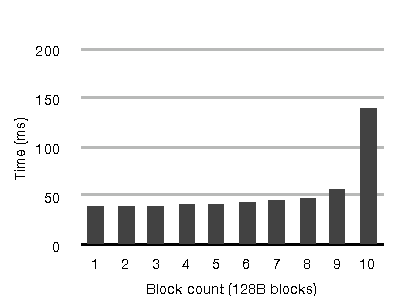
\includegraphics{client_field_count_new} \\
\end{center}
\end{frame}

\begin{frame}
\frametitle{Re-encryption rate at an XML gateway}
\begin{center}
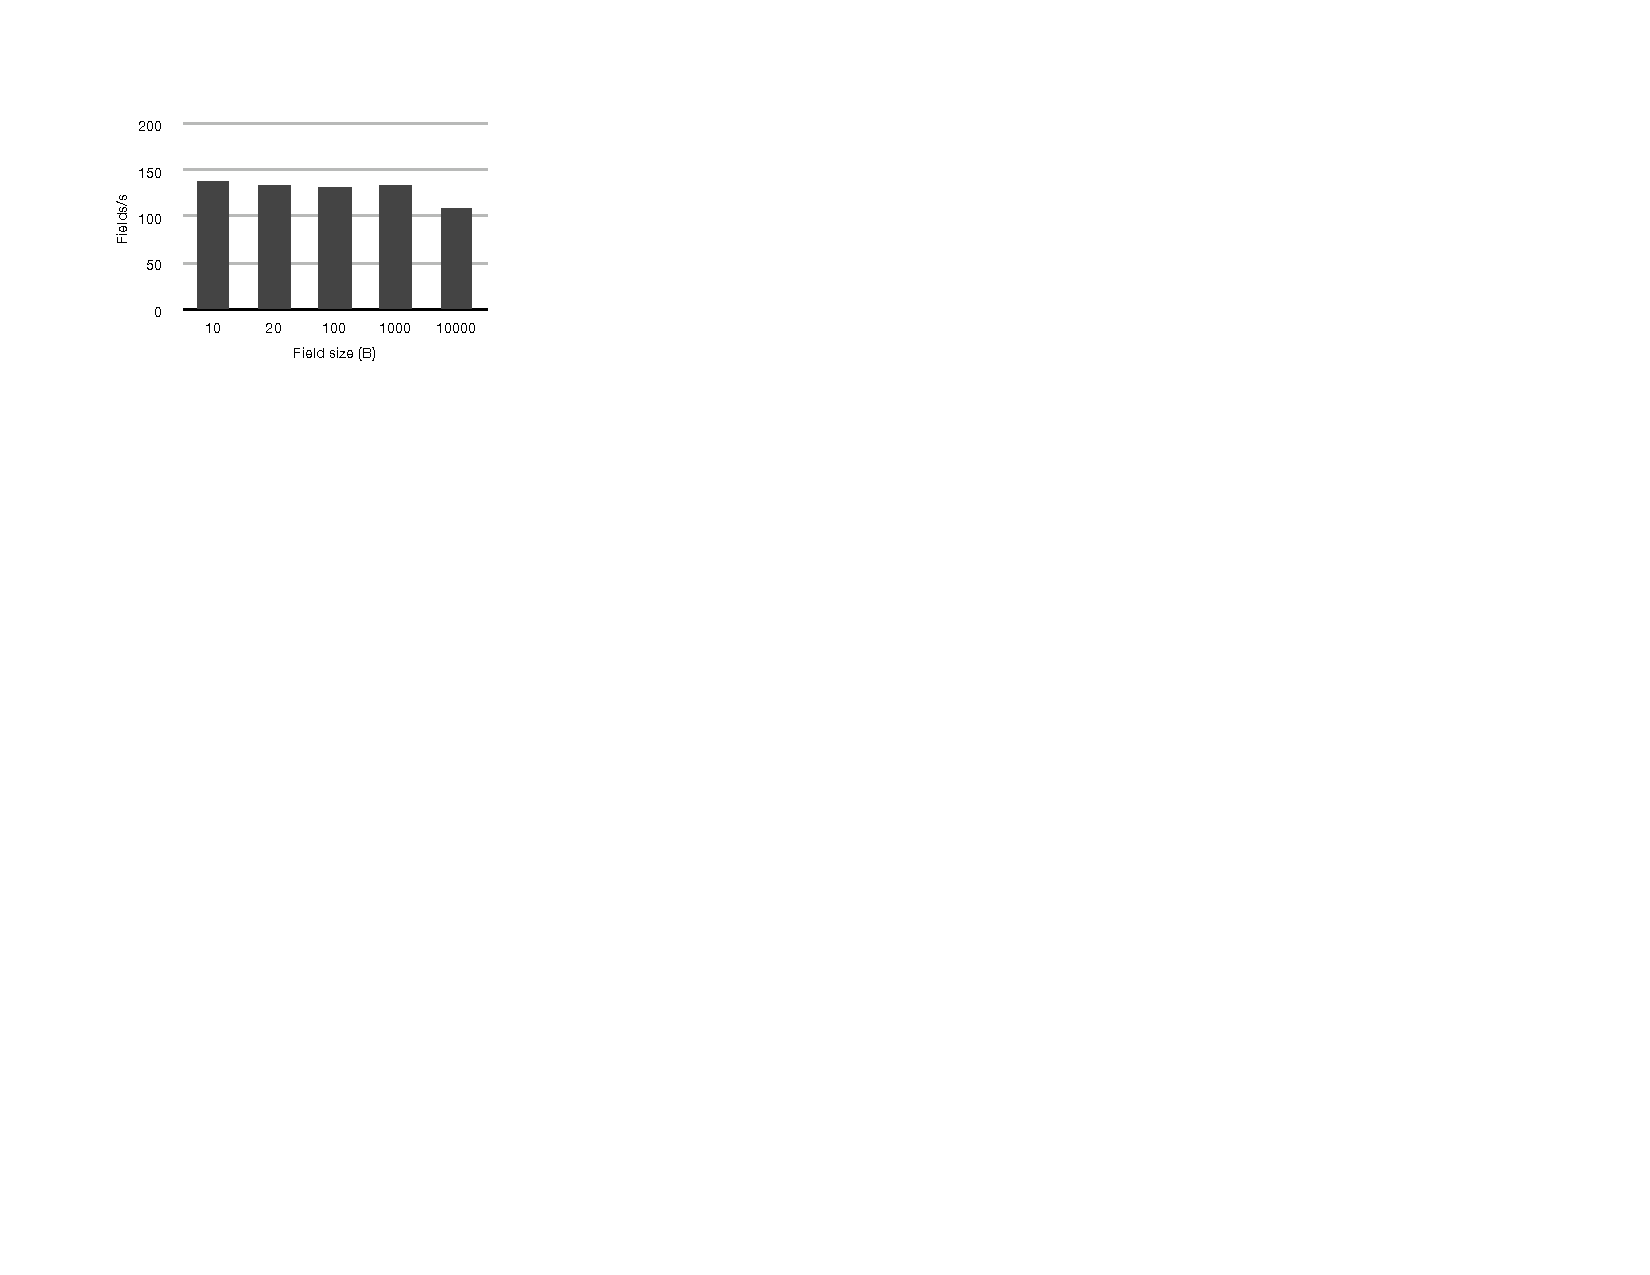
\includegraphics{server_encrypt} \\
\end{center}
\end{frame}

\begin{frame}
\frametitle{Decryption rate at an XML proxy}
\begin{center}
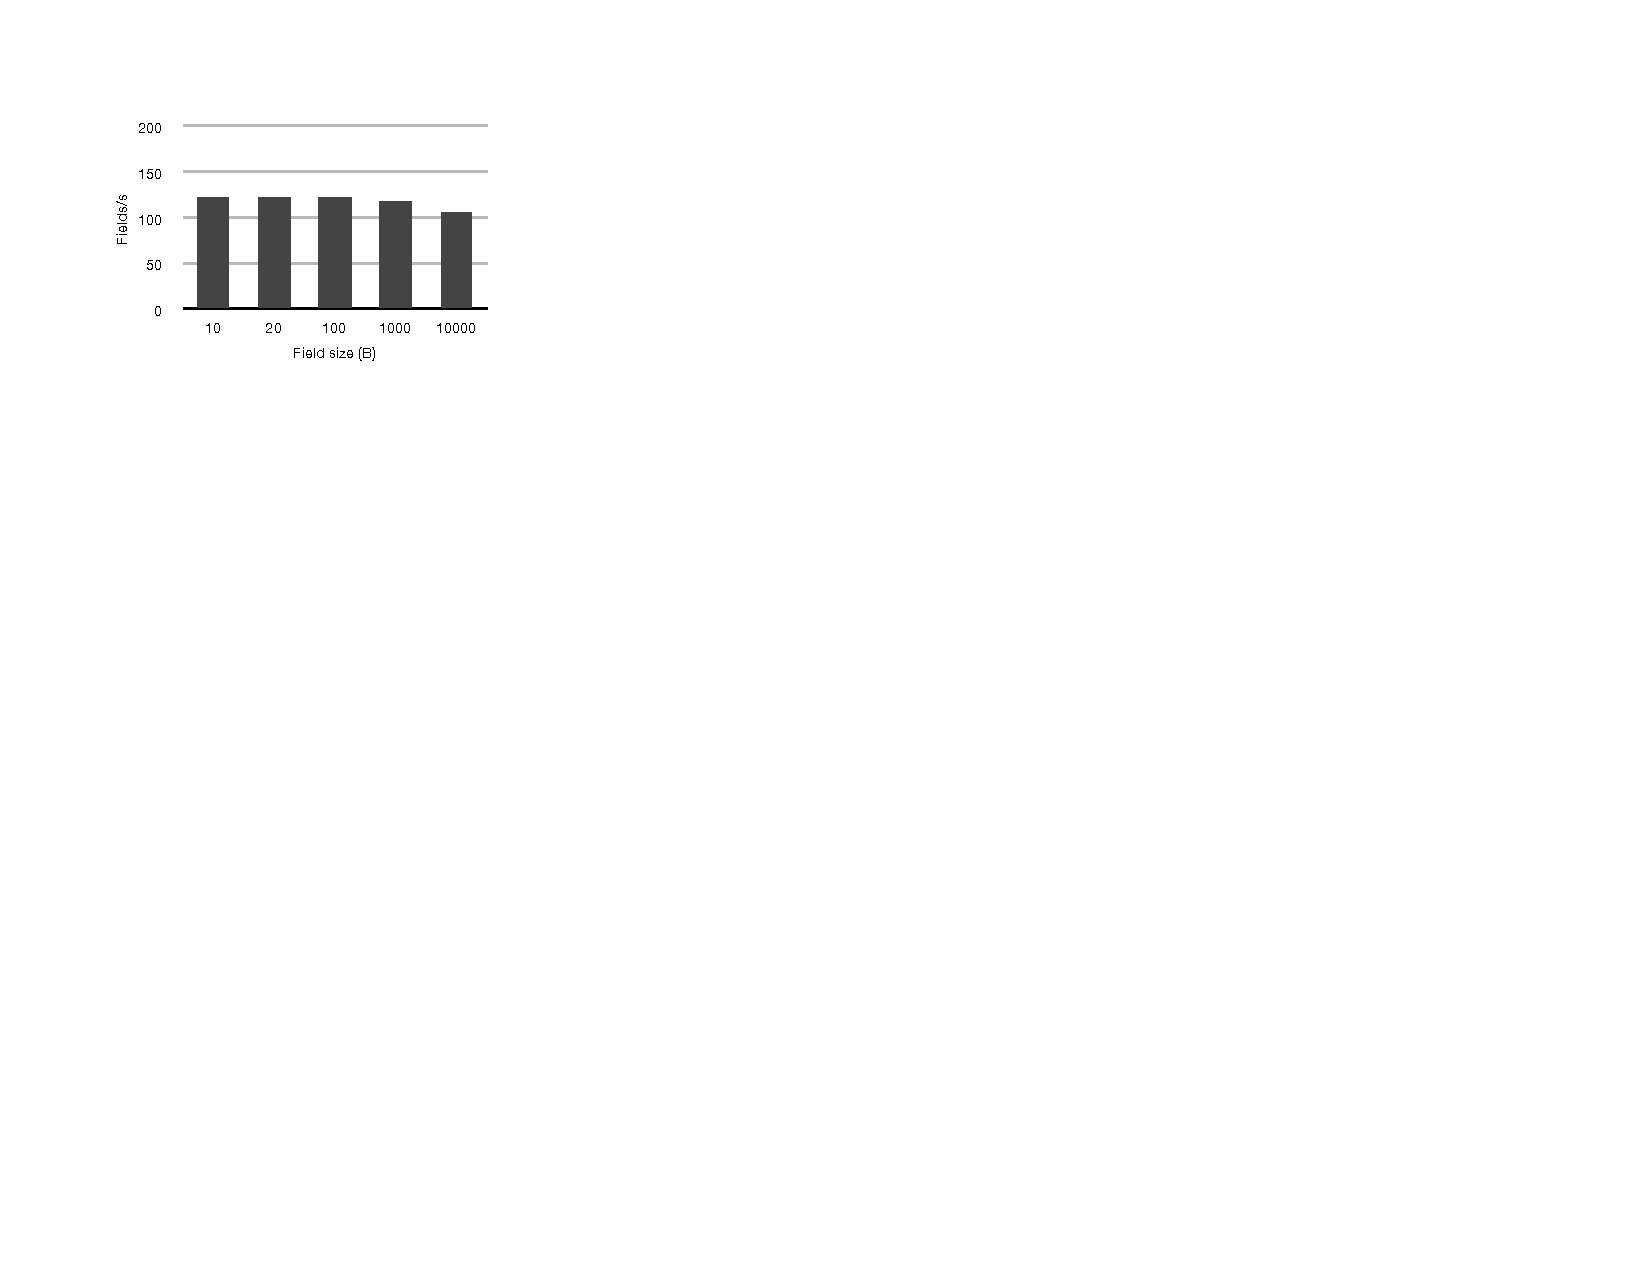
\includegraphics{server_decrypt} \\
\end{center}
\end{frame}

\section{Conclusion}
\begin{frame}
\frametitle{Conclusion}
\begin{itemize}
\item End-to-end protection to users 
\item Protection of logical architecture and partnering for SOAs
\end{itemize}
\end{frame}

\begin{thebibliography}{10}
\frametitle{References}
\bibitem[Ateniese et al., 2005]{proxy_reencryption}
G.~Ateniese, K.~Fu, M.~Green, and S.~Hohenberger.
\newblock Improved proxy re-encryption schemes with applications to secure
  distributed storage.
\newblock In {\em Proceedings of the 12th Annual Network and Distributed
  Systems Security Symposium (NDSS 2005)}, 2005.

\bibitem[Blaze et al., 1998]{atomic_proxy_reencryption}
Matt Blaze, G.~Bleumer, and M.~Strauss.
\newblock Divertible protocols and atomic proxy cryptography.
\newblock In {\em Proceedings of Eurocrypt '98}, pages 127--144, 1998.

\bibitem[Stavrou et al., 2006]{w3bcrypt}
Angelos Stavrou, Michael Locasto, and Angelos Keromytis.
\newblock W3bcrypt: Encryption as a stylesheet.
\newblock In {\em Proceedings of the 4th Applied Cryptography and Network
  Security Conference (ACNS 2006)}, pages 349--364, 2006.

\end{thebibliography}

\end{document} 
